% file: PGGL_2_8_OnConic_sims_0.tex
% created by Orbiter tikz interface
% creation date: Sat Dec 19 23:54:03 MST 2020
% DeviceCoordinates 0 0 1000000 1000000
% UserCoordinates 0 0 10000 10000
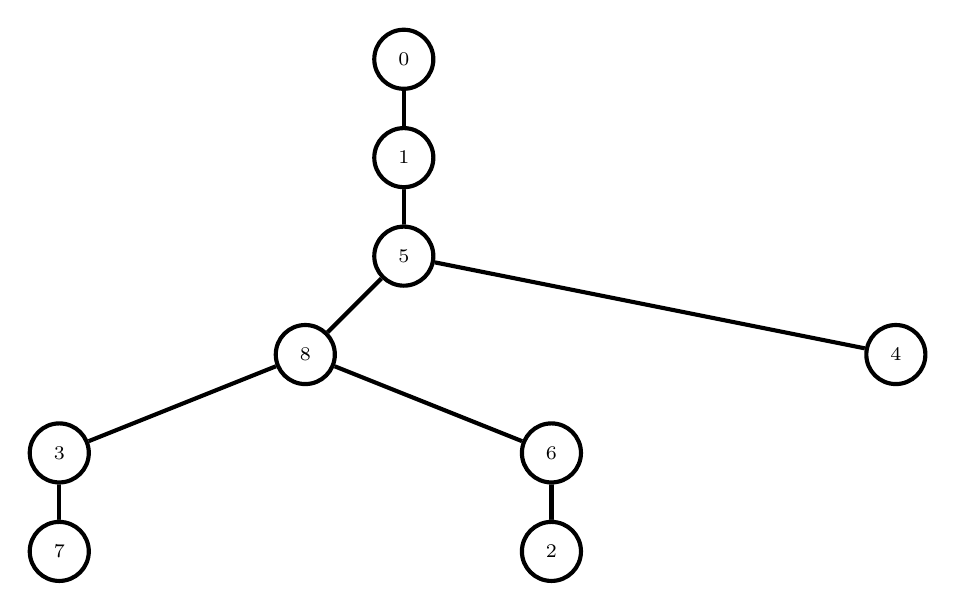
\begin{tikzpicture}[scale=0.45,line width = 1.5pt]
\draw [] (16.6667,31.9433) -- (16.6667,29.1667);
\draw [] (16.6667,29.1667) -- (16.6667,26.3867);
\draw [] (16.6667,26.3867) -- (13.8867,23.61);
\draw [] (16.6667,26.3867) -- (30.5533,23.61);
\draw [] (13.8867,23.61) -- (6.94333,20.8333);
\draw [] (13.8867,23.61) -- (20.8333,20.8333);
\draw [] (6.94333,20.8333) -- (6.94333,18.0533);
\draw [] (20.8333,20.8333) -- (20.8333,18.0533);
\filldraw[color=white] (16.6667,31.9433) circle [radius = 0.833333cm];
\draw (16.6667,31.9433) circle [radius = 0.833333cm];
\draw (16.6667,31.9433) node{{\scriptsize 0}};
\filldraw[color=white] (16.6667,29.1667) circle [radius = 0.833333cm];
\draw (16.6667,29.1667) circle [radius = 0.833333cm];
\draw (16.6667,29.1667) node{{\scriptsize 1}};
\filldraw[color=white] (16.6667,26.3867) circle [radius = 0.833333cm];
\draw (16.6667,26.3867) circle [radius = 0.833333cm];
\draw (16.6667,26.3867) node{{\scriptsize 5}};
\filldraw[color=white] (13.8867,23.61) circle [radius = 0.833333cm];
\draw (13.8867,23.61) circle [radius = 0.833333cm];
\draw (13.8867,23.61) node{{\scriptsize 8}};
\filldraw[color=white] (30.5533,23.61) circle [radius = 0.833333cm];
\draw (30.5533,23.61) circle [radius = 0.833333cm];
\draw (30.5533,23.61) node{{\scriptsize 4}};
\filldraw[color=white] (6.94333,20.8333) circle [radius = 0.833333cm];
\draw (6.94333,20.8333) circle [radius = 0.833333cm];
\draw (6.94333,20.8333) node{{\scriptsize 3}};
\filldraw[color=white] (20.8333,20.8333) circle [radius = 0.833333cm];
\draw (20.8333,20.8333) circle [radius = 0.833333cm];
\draw (20.8333,20.8333) node{{\scriptsize 6}};
\filldraw[color=white] (6.94333,18.0533) circle [radius = 0.833333cm];
\draw (6.94333,18.0533) circle [radius = 0.833333cm];
\draw (6.94333,18.0533) node{{\scriptsize 7}};
\filldraw[color=white] (20.8333,18.0533) circle [radius = 0.833333cm];
\draw (20.8333,18.0533) circle [radius = 0.833333cm];
\draw (20.8333,18.0533) node{{\scriptsize 2}};
\end{tikzpicture}
